% Created by tikzDevice version 0.6.2-92-0ad2792 on 2012-09-27 11:44:32
% !TEX encoding = UTF-8 Unicode
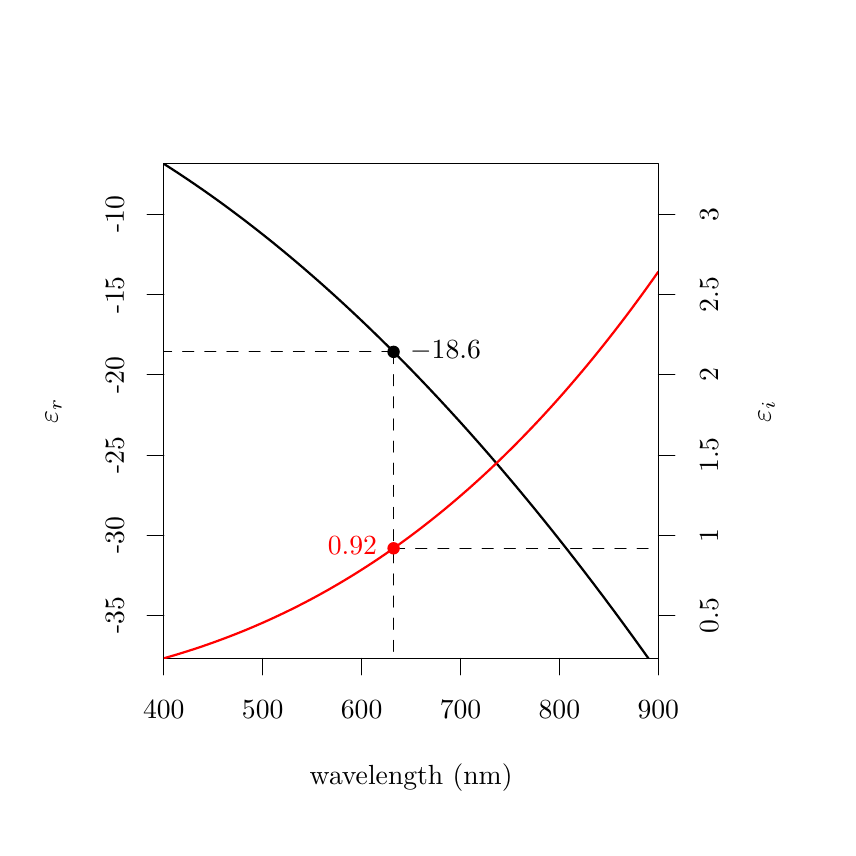
\begin{tikzpicture}[x=1pt,y=1pt]
\definecolor[named]{fillColor}{rgb}{1.00,1.00,1.00}
\path[use as bounding box,fill=fillColor,fill opacity=0.00] (0,0) rectangle (289.08,289.08);
\begin{scope}
\path[clip] (  0.00,  0.00) rectangle (289.08,289.08);
\definecolor[named]{drawColor}{rgb}{0.00,0.00,0.00}

\path[draw=drawColor,line width= 0.4pt,line join=round,line cap=round] ( 49.20, 61.20) -- (227.88, 61.20);

\path[draw=drawColor,line width= 0.4pt,line join=round,line cap=round] ( 49.20, 61.20) -- ( 49.20, 55.20);

\path[draw=drawColor,line width= 0.4pt,line join=round,line cap=round] ( 84.94, 61.20) -- ( 84.94, 55.20);

\path[draw=drawColor,line width= 0.4pt,line join=round,line cap=round] (120.67, 61.20) -- (120.67, 55.20);

\path[draw=drawColor,line width= 0.4pt,line join=round,line cap=round] (156.41, 61.20) -- (156.41, 55.20);

\path[draw=drawColor,line width= 0.4pt,line join=round,line cap=round] (192.14, 61.20) -- (192.14, 55.20);

\path[draw=drawColor,line width= 0.4pt,line join=round,line cap=round] (227.88, 61.20) -- (227.88, 55.20);

\node[text=drawColor,anchor=base,inner sep=0pt, outer sep=0pt, scale=  1.00] at ( 49.20, 39.60) {400};

\node[text=drawColor,anchor=base,inner sep=0pt, outer sep=0pt, scale=  1.00] at ( 84.94, 39.60) {500};

\node[text=drawColor,anchor=base,inner sep=0pt, outer sep=0pt, scale=  1.00] at (120.67, 39.60) {600};

\node[text=drawColor,anchor=base,inner sep=0pt, outer sep=0pt, scale=  1.00] at (156.41, 39.60) {700};

\node[text=drawColor,anchor=base,inner sep=0pt, outer sep=0pt, scale=  1.00] at (192.14, 39.60) {800};

\node[text=drawColor,anchor=base,inner sep=0pt, outer sep=0pt, scale=  1.00] at (227.88, 39.60) {900};

\path[draw=drawColor,line width= 0.4pt,line join=round,line cap=round] ( 49.20, 76.68) -- ( 49.20,221.56);

\path[draw=drawColor,line width= 0.4pt,line join=round,line cap=round] ( 49.20, 76.68) -- ( 43.20, 76.68);

\path[draw=drawColor,line width= 0.4pt,line join=round,line cap=round] ( 49.20,105.66) -- ( 43.20,105.66);

\path[draw=drawColor,line width= 0.4pt,line join=round,line cap=round] ( 49.20,134.63) -- ( 43.20,134.63);

\path[draw=drawColor,line width= 0.4pt,line join=round,line cap=round] ( 49.20,163.61) -- ( 43.20,163.61);

\path[draw=drawColor,line width= 0.4pt,line join=round,line cap=round] ( 49.20,192.59) -- ( 43.20,192.59);

\path[draw=drawColor,line width= 0.4pt,line join=round,line cap=round] ( 49.20,221.56) -- ( 43.20,221.56);

\node[text=drawColor,rotate= 90.00,anchor=base,inner sep=0pt, outer sep=0pt, scale=  1.00] at ( 34.80, 76.68) {-35};

\node[text=drawColor,rotate= 90.00,anchor=base,inner sep=0pt, outer sep=0pt, scale=  1.00] at ( 34.80,105.66) {-30};

\node[text=drawColor,rotate= 90.00,anchor=base,inner sep=0pt, outer sep=0pt, scale=  1.00] at ( 34.80,134.63) {-25};

\node[text=drawColor,rotate= 90.00,anchor=base,inner sep=0pt, outer sep=0pt, scale=  1.00] at ( 34.80,163.61) {-20};

\node[text=drawColor,rotate= 90.00,anchor=base,inner sep=0pt, outer sep=0pt, scale=  1.00] at ( 34.80,192.59) {-15};

\node[text=drawColor,rotate= 90.00,anchor=base,inner sep=0pt, outer sep=0pt, scale=  1.00] at ( 34.80,221.56) {-10};

\path[draw=drawColor,line width= 0.4pt,line join=round,line cap=round] ( 49.20, 61.20) --
	(227.88, 61.20) --
	(227.88,239.88) --
	( 49.20,239.88) --
	( 49.20, 61.20);
\end{scope}
\begin{scope}
\path[clip] ( 49.20, 61.20) rectangle (227.88,239.88);
\definecolor[named]{drawColor}{rgb}{0.00,0.00,0.00}

\path[draw=drawColor,line width= 0.8pt,line join=round,line cap=round] ( 49.20,239.88) --
	( 51.00,238.73) --
	( 52.81,237.56) --
	( 54.61,236.38) --
	( 56.42,235.18) --
	( 58.22,233.97) --
	( 60.03,232.74) --
	( 61.83,231.50) --
	( 63.64,230.25) --
	( 65.44,228.98) --
	( 67.25,227.70) --
	( 69.05,226.40) --
	( 70.86,225.09) --
	( 72.66,223.76) --
	( 74.47,222.42) --
	( 76.27,221.06) --
	( 78.08,219.70) --
	( 79.88,218.31) --
	( 81.69,216.91) --
	( 83.49,215.50) --
	( 85.30,214.07) --
	( 87.10,212.63) --
	( 88.91,211.18) --
	( 90.71,209.71) --
	( 92.52,208.22) --
	( 94.32,206.72) --
	( 96.13,205.21) --
	( 97.93,203.68) --
	( 99.74,202.14) --
	(101.54,200.58) --
	(103.35,199.01) --
	(105.15,197.43) --
	(106.96,195.83) --
	(108.76,194.21) --
	(110.56,192.59) --
	(112.37,190.94) --
	(114.17,189.29) --
	(115.98,187.61) --
	(117.78,185.93) --
	(119.59,184.23) --
	(121.39,182.52) --
	(123.20,180.79) --
	(125.00,179.04) --
	(126.81,177.29) --
	(128.61,175.52) --
	(130.42,173.73) --
	(132.22,171.93) --
	(134.03,170.11) --
	(135.83,168.29) --
	(137.64,166.44) --
	(139.44,164.59) --
	(141.25,162.71) --
	(143.05,160.83) --
	(144.86,158.93) --
	(146.66,157.01) --
	(148.47,155.09) --
	(150.27,153.14) --
	(152.08,151.18) --
	(153.88,149.21) --
	(155.69,147.23) --
	(157.49,145.23) --
	(159.30,143.21) --
	(161.10,141.18) --
	(162.91,139.14) --
	(164.71,137.08) --
	(166.52,135.01) --
	(168.32,132.93) --
	(170.12,130.83) --
	(171.93,128.71) --
	(173.73,126.58) --
	(175.54,124.44) --
	(177.34,122.29) --
	(179.15,120.11) --
	(180.95,117.93) --
	(182.76,115.73) --
	(184.56,113.52) --
	(186.37,111.29) --
	(188.17,109.05) --
	(189.98,106.79) --
	(191.78,104.52) --
	(193.59,102.23) --
	(195.39, 99.94) --
	(197.20, 97.62) --
	(199.00, 95.30) --
	(200.81, 92.95) --
	(202.61, 90.60) --
	(204.42, 88.23) --
	(206.22, 85.84) --
	(208.03, 83.45) --
	(209.83, 81.03) --
	(211.64, 78.61) --
	(213.44, 76.17) --
	(215.25, 73.71) --
	(217.05, 71.24) --
	(218.86, 68.76) --
	(220.66, 66.26) --
	(222.47, 63.75) --
	(224.27, 61.23) --
	(226.08, 58.69) --
	(227.88, 56.13);
\definecolor[named]{drawColor}{rgb}{1.00,0.00,0.00}

\path[draw=drawColor,line width= 0.8pt,line join=round,line cap=round] ( 49.20, 61.20) --
	( 51.00, 61.72) --
	( 52.81, 62.25) --
	( 54.61, 62.79) --
	( 56.42, 63.35) --
	( 58.22, 63.92) --
	( 60.03, 64.50) --
	( 61.83, 65.10) --
	( 63.64, 65.71) --
	( 65.44, 66.34) --
	( 67.25, 66.98) --
	( 69.05, 67.64) --
	( 70.86, 68.31) --
	( 72.66, 68.99) --
	( 74.47, 69.69) --
	( 76.27, 70.40) --
	( 78.08, 71.13) --
	( 79.88, 71.88) --
	( 81.69, 72.64) --
	( 83.49, 73.42) --
	( 85.30, 74.21) --
	( 87.10, 75.02) --
	( 88.91, 75.85) --
	( 90.71, 76.69) --
	( 92.52, 77.55) --
	( 94.32, 78.42) --
	( 96.13, 79.31) --
	( 97.93, 80.22) --
	( 99.74, 81.15) --
	(101.54, 82.09) --
	(103.35, 83.05) --
	(105.15, 84.03) --
	(106.96, 85.03) --
	(108.76, 86.04) --
	(110.56, 87.08) --
	(112.37, 88.13) --
	(114.17, 89.20) --
	(115.98, 90.29) --
	(117.78, 91.39) --
	(119.59, 92.52) --
	(121.39, 93.67) --
	(123.20, 94.83) --
	(125.00, 96.02) --
	(126.81, 97.22) --
	(128.61, 98.44) --
	(130.42, 99.69) --
	(132.22,100.95) --
	(134.03,102.24) --
	(135.83,103.54) --
	(137.64,104.87) --
	(139.44,106.21) --
	(141.25,107.58) --
	(143.05,108.97) --
	(144.86,110.38) --
	(146.66,111.81) --
	(148.47,113.26) --
	(150.27,114.73) --
	(152.08,116.23) --
	(153.88,117.75) --
	(155.69,119.29) --
	(157.49,120.85) --
	(159.30,122.43) --
	(161.10,124.04) --
	(162.91,125.67) --
	(164.71,127.32) --
	(166.52,129.00) --
	(168.32,130.70) --
	(170.12,132.42) --
	(171.93,134.17) --
	(173.73,135.94) --
	(175.54,137.74) --
	(177.34,139.55) --
	(179.15,141.40) --
	(180.95,143.27) --
	(182.76,145.16) --
	(184.56,147.07) --
	(186.37,149.01) --
	(188.17,150.98) --
	(189.98,152.97) --
	(191.78,154.99) --
	(193.59,157.03) --
	(195.39,159.10) --
	(197.20,161.20) --
	(199.00,163.32) --
	(200.81,165.46) --
	(202.61,167.63) --
	(204.42,169.83) --
	(206.22,172.06) --
	(208.03,174.31) --
	(209.83,176.59) --
	(211.64,178.90) --
	(213.44,181.23) --
	(215.25,183.59) --
	(217.05,185.98) --
	(218.86,188.40) --
	(220.66,190.84) --
	(222.47,193.31) --
	(224.27,195.81) --
	(226.08,198.34) --
	(227.88,200.90);
\end{scope}
\begin{scope}
\path[clip] (  0.00,  0.00) rectangle (289.08,289.08);
\definecolor[named]{drawColor}{rgb}{0.00,0.00,0.00}

\path[draw=drawColor,line width= 0.4pt,line join=round,line cap=round] (227.88, 76.68) -- (227.88,221.56);

\path[draw=drawColor,line width= 0.4pt,line join=round,line cap=round] (227.88, 76.68) -- (233.88, 76.68);

\path[draw=drawColor,line width= 0.4pt,line join=round,line cap=round] (227.88,105.66) -- (233.88,105.66);

\path[draw=drawColor,line width= 0.4pt,line join=round,line cap=round] (227.88,134.63) -- (233.88,134.63);

\path[draw=drawColor,line width= 0.4pt,line join=round,line cap=round] (227.88,163.61) -- (233.88,163.61);

\path[draw=drawColor,line width= 0.4pt,line join=round,line cap=round] (227.88,192.59) -- (233.88,192.59);

\path[draw=drawColor,line width= 0.4pt,line join=round,line cap=round] (227.88,221.56) -- (233.88,221.56);

\node[text=drawColor,rotate= 90.00,anchor=base,inner sep=0pt, outer sep=0pt, scale=  1.00] at (249.48, 76.68) {0.5};

\node[text=drawColor,rotate= 90.00,anchor=base,inner sep=0pt, outer sep=0pt, scale=  1.00] at (249.48,105.66) {1};

\node[text=drawColor,rotate= 90.00,anchor=base,inner sep=0pt, outer sep=0pt, scale=  1.00] at (249.48,134.63) {1.5};

\node[text=drawColor,rotate= 90.00,anchor=base,inner sep=0pt, outer sep=0pt, scale=  1.00] at (249.48,163.61) {2};

\node[text=drawColor,rotate= 90.00,anchor=base,inner sep=0pt, outer sep=0pt, scale=  1.00] at (249.48,192.59) {2.5};

\node[text=drawColor,rotate= 90.00,anchor=base,inner sep=0pt, outer sep=0pt, scale=  1.00] at (249.48,221.56) {3};
\end{scope}
\begin{scope}
\path[clip] (  0.00,  0.00) rectangle (289.08,289.08);
\definecolor[named]{drawColor}{rgb}{0.00,0.00,0.00}

\node[text=drawColor,anchor=base,inner sep=0pt, outer sep=0pt, scale=  1.00] at (138.54, 15.60) {wavelength (nm)};

\node[text=drawColor,rotate= 90.00,anchor=base,inner sep=0pt, outer sep=0pt, scale=  1.00] at ( 10.80,150.54) {$\varepsilon_r$};
\end{scope}
\begin{scope}
\path[clip] (  0.00,  0.00) rectangle (289.08,289.08);
\definecolor[named]{drawColor}{rgb}{0.00,0.00,0.00}

\node[text=drawColor,rotate= 90.00,anchor=base,inner sep=0pt, outer sep=0pt, scale=  1.00] at (268.47,150.54) {$\varepsilon_i$};
\end{scope}
\begin{scope}
\path[clip] ( 49.20, 61.20) rectangle (227.88,239.88);
\definecolor[named]{drawColor}{rgb}{0.00,0.00,0.00}

\path[draw=drawColor,line width= 0.4pt,dash pattern=on 4pt off 4pt ,line join=round,line cap=round] (132.22, 47.70) --
	(132.22, 54.24) --
	(132.22, 60.78) --
	(132.22, 67.32) --
	(132.22, 73.86) --
	(132.22, 80.39) --
	(132.22, 86.93) --
	(132.22, 93.47) --
	(132.22,100.01) --
	(132.22,106.55) --
	(132.22,113.09) --
	(132.22,119.62) --
	(132.22,126.16) --
	(132.22,132.70) --
	(132.22,139.24) --
	(132.22,145.78) --
	(132.22,152.31) --
	(132.22,158.85) --
	(132.22,165.39) --
	(132.22,171.93);

\path[draw=drawColor,line width= 0.4pt,dash pattern=on 4pt off 4pt ,line join=round,line cap=round] (132.22,100.95) --
	(139.14,100.95) --
	(146.05,100.95) --
	(152.97,100.95) --
	(159.88,100.95) --
	(166.80,100.95) --
	(173.72,100.95) --
	(180.63,100.95) --
	(187.55,100.95) --
	(194.46,100.95) --
	(201.38,100.95) --
	(208.29,100.95) --
	(215.21,100.95) --
	(222.12,100.95) --
	(229.04,100.95) --
	(235.95,100.95) --
	(242.87,100.95) --
	(249.79,100.95) --
	(256.70,100.95) --
	(263.62,100.95);

\path[draw=drawColor,line width= 0.4pt,dash pattern=on 4pt off 4pt ,line join=round,line cap=round] (  0.00,171.93) --
	(  1.40,171.93) --
	( 13.29,171.93) --
	( 25.19,171.93) --
	( 37.08,171.93) --
	( 48.97,171.93) --
	( 60.87,171.93) --
	( 72.76,171.93) --
	( 84.65,171.93) --
	( 96.54,171.93) --
	(108.44,171.93) --
	(120.33,171.93) --
	(132.22,171.93);
\definecolor[named]{fillColor}{rgb}{0.00,0.00,0.00}

\path[fill=fillColor] (132.22,171.93) circle (  2.25);
\definecolor[named]{fillColor}{rgb}{1.00,0.00,0.00}

\path[fill=fillColor] (132.22,100.95) circle (  2.25);

\node[text=drawColor,anchor=base west,inner sep=0pt, outer sep=0pt, scale=  1.00] at (138.22,169.63) {$-18.6$};
\definecolor[named]{drawColor}{rgb}{1.00,0.00,0.00}

\node[text=drawColor,anchor=base east,inner sep=0pt, outer sep=0pt, scale=  1.00] at (126.22, 98.66) {$0.92$};
\end{scope}
\end{tikzpicture}
